% TCC: História da Engenharia de Reservatórios (versão ISPTEC - OTIMIZADA)
\PassOptionsToPackage{brazilian}{babel}
\documentclass[12pt,a4paper,oneside,brazilian,sumario=tradicional]{abntex2}

% =========================
% PACOTES ESSENCIAIS
% =========================
\usepackage[T1]{fontenc}
\usepackage[utf8]{inputenc}
\usepackage{times}
\renewcommand{\familydefault}{\rmdefault}

\usepackage{geometry}
\geometry{a4paper,left=3cm,right=2cm,top=3cm,bottom=2cm}

\usepackage{setspace}
\OnehalfSpacing

\usepackage{indentfirst}
\setlength{\parindent}{1.25cm}

\usepackage{microtype}
\usepackage{emptypage}

% =========================
% FIGURAS E TABELAS (OTIMIZADO - SEM WRAPFIGURE)
% =========================
\usepackage{graphicx}
\usepackage{grffile}
\usepackage{wrapfig}
\graphicspath{{figuras/}}

% Controle otimizado para wrapfigure
\usepackage{float}

% Espaçamento específico para wrapfigure
\setlength{\intextsep}{8pt}
\setlength{\textfloatsep}{8pt}

\usepackage{booktabs}
\usepackage{longtable}
\usepackage{array}
\usepackage{multirow}

% Caption otimizado conforme ABNT (tamanho 10)
\usepackage{caption}
\captionsetup{
  font=footnotesize,
  labelfont=bf,
  justification=centering,
  skip=6pt
}

% Comando customizado para fonte - tamanho 10 conforme ABNT
\renewcommand{\fonte}[1]{\vspace{1pt}\par\noindent\fontsize{10}{10}\selectfont Fonte: #1\normalsize}

% =========================
% MATEMÁTICA
% =========================
\usepackage{amsmath}
\usepackage{amssymb}
\usepackage{amsfonts}

% =========================
% UTILITÁRIOS
% =========================
\usepackage{hyperref}
\usepackage{xcolor}
\usepackage{enumitem}
\usepackage{lastpage}

% =========================
% CONFIGURAÇÃO DE TÍTULOS - TIMES NEW ROMAN
% =========================
\usepackage{titlesec}
\titleformat{\chapter}{\rmfamily\bfseries\Large}{\thechapter\hspace{1em}}{0pt}{}
\titleformat{\section}{\rmfamily\bfseries\large}{\thesection\hspace{0.5em}}{0pt}{}
\titleformat{\subsection}{\rmfamily\bfseries}{\thesubsection\hspace{0.5em}}{0pt}{}
\titleformat{\subsubsection}{\rmfamily}{\thesubsubsection\hspace{0.5em}}{0pt}{}

% Customização de títulos automáticos - ABNT em Times New Roman
\renewcommand{\resumoname}{\rmfamily\textbf{Resumo}}
\renewcommand{\abstractname}{\rmfamily\textbf{Abstract}}
\renewcommand{\contentsname}{\rmfamily\textbf{Sumário}}
\renewcommand{\listfigurename}{\rmfamily\textbf{Lista de Figuras}}
\renewcommand{\listtablename}{\rmfamily\textbf{Lista de Tabelas}}
\renewcommand{\bibname}{\rmfamily\textbf{Referências}}

% =========================
% BIBLIOGRAFIA
% =========================
% Usando estilo ABNT para referências

% Configurações ABNT: números arábicos no canto superior direito a partir da introdução
\hypersetup{
  pdftitle={História da Engenharia de Reservatórios},
  pdfauthor={Rocélio Da Silva, Marquinha Marcos, Arlindo Jamba et al},
  colorlinks=true,
  linkcolor=black,
  citecolor=black,
  urlcolor=black
}

% Compatibilidades
\usepackage{url}
\providecommand{\htmladdnormallink}[2]{\href{#2}{#1}}

% Dados do trabalho (preencha conforme necessário)
\titulo{A história de engenharia de reservatórios de petróleo}
\autor{Rocélio Da Silva (20220001) \\ Marquinha Marcos (20200721) \\ Arlindo Jamba (20222182) \\ Nadir Manuel (20211333) \\ Manuel Braz (20222320) \\ Paulo Isaac Abel (20220918) \\ Cristina Bongue (20221099)}
\orientador{Prof.\ Geraldo André Raposo Ramos}
\instituicao{Instituto Superior Politécnico de Tecnologias e Ciências -- ISPTEC\\Departamento de Geociências\\Curso de Engenharia de Petróleo}
\local{Luanda -- Angola}
\data{2026}
\tipotrabalho{Trabalho de Avaliação Contínua}
\preambulo{Trabalho investigativo apresentado ao Curso de Engenharia de Petróleo do Departamento de Geociências do Instituto Superior Politécnico de Tecnologias e Ciências (ISPTEC) como avaliação contínua na disciplina de Engenharia de Reservatórios.}

\begin{document}
\frenchspacing
\pretextual

% ===========================
% CAPA CUSTOMIZADA CONFORME NORMAS ISPTEC
% ===========================
\thispagestyle{empty}
\begin{center}
  % Logo ISPTEC no topo
  \vspace*{0.5cm}
  
\includegraphics[width=3.5cm]{logo isptec.png}
  
  \vspace*{0.8cm}
  
  % Cabeçalho com dados da instituição
  {\large\bfseries DEPARTAMENTO DE GEOCIÊNCIAS E TECNOLOGIAS}
  
  \vspace*{0.3cm}
  
  {\large\bfseries CURSO DE ENGENHARIA DE PETRÓLEO}
  
  \vspace*{2.0cm}
  
  % Nome do autor
  {\large\bfseries GRUPO 5}
  
  \vspace*{1.5cm}
  
  % Título do trabalho
  {\bfseries\Large A HISTÓRIA DA ENGENHARIA DE RESERVATÓRIOS DE PETRÓLEO}
  
  \vspace*{3.0cm}
  
  % Espaço para o trabalho
  ~
  
  \vfill
  
  % Rodapé com local e data
  {\large\bfseries Luanda}
  
  {\large\bfseries 2026}
  
  \vspace*{0.5cm}
\end{center}

% Configurar a página para não contar como numerada
\clearpage
\phantomsection

% ===========================
% FOLHA DE ROSTO
% ===========================
\thispagestyle{empty}
\begin{center}
  
  \vspace*{2.0cm}
  
  {\large\bfseries GRUPO 5}
  
  \vspace*{1.5cm}
  
  {\bfseries\Large A HISTÓRIA DA ENGENHARIA DE RESERVATÓRIOS DE PETRÓLEO}
  
  \vspace*{2.0cm}
  
\end{center}

\hspace*{3.5cm}\begin{minipage}[t]{9.5cm}
Trabalho investigativo apresentado ao Curso de Engenharia de Petróleo do Departamento de Geociências do Instituto Superior Politécnico de Tecnologias e Ciências (ISPTEC) como avaliação contínua na disciplina de Engenharia de Reservatórios.

\vspace*{1.0cm}

\noindent Orientador: Prof.\ Geraldo André Raposo Ramos
\end{minipage}

\vspace*{2.0cm}

\begin{center}
  {\large\bfseries Luanda}
  
  {\large\bfseries 2026}
\end{center}

\clearpage

% Folha de aprovação simplificada
\begin{folhadeaprovacao}
  \thispagestyle{empty}
  \begin{center}
    {\large\bfseries\MakeUppercase{\imprimirautor}}
    \vspace*{1cm}
    \begin{center}
      \bfseries\large\MakeUppercase{\imprimirtitulo}
    \end{center}
    \vspace*{1cm}
    \hspace{.38\textwidth}
    \begin{minipage}{.56\textwidth}
      \imprimirpreambulo
    \end{minipage}
    \vspace*{1cm}
  \end{center}

  Trabalho avaliado em \underline{\hspace{2.0cm}} de \underline{\hspace{3.5cm}} de \underline{\hspace{1.2cm}}

  \vspace{1.5cm}
  \assinatura{\textbf{\imprimirorientador} \\ Prof. Orientador}

  \begin{center}
    \imprimirlocal, \imprimirdata
  \end{center}
\end{folhadeaprovacao}







% Resumo e abstract
\setlength{\absparsep}{18pt}
\begin{resumo}
A Engenharia de Reservatórios de Petróleo é uma das disciplinas mais fascinantes e intelectualmente rigorosas da engenharia moderna: é ela que permite saber quanto petróleo existe no subsolo, quanto dele é possível extrair economicamente e de que maneira fazê-lo com eficiência técnica. Este trabalho investigativo traça a evolução histórica dessa disciplina — desde as práticas artesanais da Antiguidade até os sofisticados sistemas de Inteligência Artificial do século XXI —, reconstruindo como se transformou de um ofício empírico numa ciência quantitativa de rigor comparável ao das engenharias mais avançadas. A metodologia empregada consistiu em revisão bibliográfica qualitativa e analítica, com base em obras clássicas e contemporâneas de referência internacional. Os resultados revelam que a evolução da disciplina se organizou em quatro fases paradigmáticas claramente delimitadas: a \textbf{era empírica} (Antiguidade ao século XVIII), marcada pela ausência de fundamentação científica; a \textbf{era da fundamentação teórica} (século XIX ao início do século XX), ancorada na Lei de Darcy (1856) e na sistematização matemática do escoamento em meios porosos; a \textbf{era da consolidação científica} (século XX), durante a qual se desenvolveram o método do balanço de materiais, a análise de pressão transiente e os primeiros simuladores computacionais; e a \textbf{era digital e avançada} (século XXI), definida pela integração de Internet das Coisas (IoT), aprendizado de máquina e técnicas de Recuperação Avançada de Petróleo (EOR). Conclui-se que a Engenharia de Reservatórios exemplifica, de maneira paradigmática, a transição da engenharia como ofício artesanal para uma ciência rigorosa de modelagem e otimização de sistemas físicos complexos.

\vspace{\onelineskip}
\noindent
\textbf{Palavras-chave}: Engenharia de Reservatórios de Petróleo. História do Petróleo. Lei de Darcy. Balanço de Materiais. Simulação Numérica de Reservatórios. Análise de Pressão Transiente. Recuperação Avançada de Petróleo (EOR). Inteligência Artificial.
\end{resumo}

\begin{resumo}[Abstract]
\begin{otherlanguage*}{english}
Petroleum Reservoir Engineering is one of the most intellectually compelling and strategically vital disciplines in modern engineering: it is the science that determines how much oil exists in the subsurface, how much can be economically recovered, and by what technical means. This investigative work traces the historical evolution of the discipline from the artisanal practices of Antiquity to the sophisticated Artificial Intelligence-based systems of the 21st century, reconstructing how it transformed from an empirical craft into a quantitative science of comparable rigor to the most advanced engineering disciplines. The methodology consisted of a qualitative and analytical bibliographic review, drawing on classical and contemporary works from international scholarship. The results reveal that the discipline's evolution unfolded across four clearly defined paradigmatic phases: the \textbf{empirical era} (Antiquity to the 18th century), characterised by the absence of scientific foundations; the \textbf{theoretical foundation era} (19th century to the early 20th century), anchored by Darcy's Law (1856) and the mathematical systematisation of fluid flow in porous media; the \textbf{scientific consolidation era} (20th century), during which the material balance method, transient pressure analysis, and the first computational simulators were developed; and the \textbf{digital and advanced era} (21st century), defined by the integration of the Internet of Things (IoT), machine learning, and Enhanced Oil Recovery (EOR) techniques. It is concluded that Petroleum Reservoir Engineering exemplifies the historical transition of engineering from artisanal practice to a rigorous science of modelling and optimising complex physical systems.

\vspace{\onelineskip}
\noindent
\textbf{Keywords}: Petroleum Reservoir Engineering. History of Oil. Darcy's Law. Material Balance. Numerical Reservoir Simulation. Transient Pressure Analysis. Enhanced Oil Recovery (EOR). Artificial Intelligence.
\end{otherlanguage*}
\end{resumo}

% (Listas de figuras/tabelas removidas quando vazias para reduzir páginas desnecessárias)

\begin{siglas}
  \item[CCS] Captura e Armazenamento de CO\textsubscript{2}
  \item[EOR] Recuperação Avançada de Petróleo
  \item[ISPTEC] Instituto Superior Politécnico de Tecnologias e Ciências
  \item[OOIP] Original Oil In Place
\end{siglas}

\pdfbookmark[0]{\contentsname}{toc}
\tableofcontents*
\cleardoublepage

% Texto principal
\textual

\chapter{Introdução}

A Engenharia de Reservatórios é a disciplina da engenharia de petróleo responsável pela análise do fluxo de fluidos em meios porosos, pela previsão do comportamento de pressão e saturação, e pela otimização da recuperação de hidrocarbonetos. Integra modelos físicos (Lei de Darcy), modelos matemáticos (equação de difusividade, balanço de materiais) e ferramentas computacionais (simuladores numéricos) para caracterizar propriedades como permeabilidade ($k$), porosidade ($\phi$) e propriedades de fluido (PVT: pressão, volume, temperatura).

O fator de recuperação -- razão entre hidrocarbonetos produzidos e volume original em lugar -- é o objetivo central desta disciplina: ele determina tanto a viabilidade econômica de um campo quanto a duração de sua vida produtiva. Engenheiros de reservatórios trabalham ao longo de todo o ciclo de vida do campo -- avaliação, caracterização, modelação, previsão e otimização do desenvolvimento e produção.

\chapter{Objetivos}

\section{Objetivo Geral}

Investigar e descrever a evolução histórica da Engenharia de Reservatórios de Petróleo, identificando as fases paradigmáticas de seu desenvolvimento, os marcos teóricos e tecnológicos que as caracterizam, e a forma como uma disciplina empírica transformou-se numa ciência quantitativa rigorosa.

\section{Objetivos Específicos}

\begin{enumerate}[label=\alph*)]
  \item Descrever os fundamentos teóricos que estruturam o nascimento da Engenharia de Reservatórios como disciplina científica, desde a Lei de Darcy (1856) até à rigorous formulação matemática do balanço de materiais (Schilthuis, 1936) e análise de pressão transiente (Horner, 1951);
  \item Caracterizar a evolução tecnológica da disciplina através de três gerações principais: o método analítico clássico (1856-1960), a simulação numérica computacional (1960-1990), e os sistemas inteligentes baseados em dados e otimização (1990-presente);
  \item Identificar as tecnologias emergentes que redefinem a prática disciplinar no século XXI, nomeadamente Internet das Coisas, aprendizado de máquina, Recuperação Avançada de Petróleo (EOR), e o papel crítico da qualidade de dados e validação de modelos.
\end{enumerate}

\chapter{Metodologia}

Este trabalho empreende uma investigação de natureza qualitativa, histórica e bibliográfica, enquadrada no paradigma histórico-epistemológico das ciências da engenharia aplicada.

\section{Tipo de Pesquisa}

Trata-se de pesquisa exploratória e descritiva, com enfoque em reconstrução histórica da evolução disciplinar. O método é predominantemente qualitativo: análise temática e cronológica de marcos teóricos, tecnológicos e institucionais que definiram fases distintas.

\section{Fontes de Dados}

\begin{itemize}
  \item \textbf{Primárias:} Trabalhos seminais que estabeleceram marcos disciplinares (Darcy 1856, Schilthuis 1936, Horner 1951, Matthews \& Russell 1967, Dake 1978, Ahmed 2010, Rosa et al.~2006);
  \item \textbf{Secundárias:} Textbooks clássicos, artigos de revisão em periódicos internacionais (Journal of Petroleum Technology, SPE Reservoir Engineering, Petroleum Science) que documentam evolução de métodos;
  \item \textbf{Institucionais:} Contribuições de organizações internacionais (SPE -- Society of Petroleum Engineers) e associações académicas que moldaram educação profissional;
  \item \textbf{Tecnológicas:} Documentação de evolução de simuladores numéricos (ECLIPSE, CMG, INTERSECT) e plataformas de dados que exemplificam avanços na prática disciplinar.
\end{itemize}

\section{Critérios de Seleção}

\begin{enumerate}
  \item \textbf{Relevância disciplinar:} Obras que introduziram ou consolidaram metodologias hoje universalmente aceitas (Lei de Darcy, MBE, análise transiente, simulação numérica, EOR, otimização computacional);
  \item \textbf{Impacto paradigmático:} Marcos que definiram transições críticas na compreensão teórica ou capacidade prática (empirismo $\rightarrow$ ciência, analítico $\rightarrow$ computacional, determinístico $\rightarrow$ probabilístico);
  \item \textbf{Relevância global:} Documentação de como técnicas desenvolvidas numa região (EUA, Europa) difundiram-se e tornaram-se standard internacional;
  \item \textbf{Perspectiva histórica crítica:} Inclusão de limitações reconhecidas de cada era, não apenas sucessos, para facilitar lições aprendidas.
\end{enumerate}

\section{Análise e Organização}

A análise foi organizada em dois eixos complementares:

\begin{itemize}
  \item \textbf{Eixo cronológico:} História linear em quatro fases (empírica, fundamentação, consolidação, digital), cada uma caracterizada por estado do conhecimento, tecnologias dominantes, autores emblematicos e limitações epistemológicas;
  \item \textbf{Eixo temático:} Dentro de cada fase, identificação de temas transversais (teoria vs. prática, empirismo vs. rigor matemático, computação, sustentabilidade).
\end{itemize}

\section{Limitações da Pesquisa}

\begin{itemize}
  \item Acesso limitado a documentação técnica original de campos angolanos (muitos relatórios são proprietários ou confidenciais);
  \item Foco em evolução conceitual e metodológica, não em detalhes de campo específico;
  \item Horizonte até 2026; futuras descobertas tecnológicas não são cobertas;
  \item Perspectiva predominantemente técnica, com menor ênfase em aspectos sociais, políticos ou histórico-econômicos do setor.
\end{itemize}

\chapter{Justificativa}

A pertinência deste trabalho repousa em duas dimensões fundamentais e complementares: epistemológica e educacional.

\section*{Dimensão Epistemológica}

Reconstruir a história de uma disciplina científica não é mero exercício acadêmico: é reconstruir como o conhecimento humano se organiza quando confrontado com um problema técnico concreto. A Engenharia de Reservatórios exemplifica, de forma paradigmática, a transição de uma prática empírica e artesanal para uma ciência quantitativa rigorosa. Esta trajetória — de aproximadamente dois séculos — encapsula as mesmas transformações epistemológicas que caracterizaram a evolução da engenharia como disciplina moderna.

Compreender esta evolução não é luxo intelectual. Permite aos profissionais:

\begin{itemize}
  \item Reconhecer os pressupostos subjacentes a cada metodologia (Lei de Darcy: linearidade; Balanço de Materiais: conservação de massa; Simulação: discretização);
  \item Avaliar criticamente as limitações de cada abordagem e conhecer seu domínio de validade;
  \item Identificar quando uma ferramenta deixa de ser apropriada e quando transições paradigmáticas se tornam necessárias;
  \item Fundamentar inovações futuras em princípios consolidados, evitando reinvenção de soluções já exploradas.
\end{itemize}

Esta capacidade — não apenas aplicar, mas compreender a origem e evolução de métodos — é o que distingue engenheiros competentes e inovadores.



\section*{Dimensão Educacional e Profissional}

A crescente complexidade da Engenharia de Reservatórios contemporânea — com integração de Internet das Coisas, aprendizado de máquina, análise massiva de dados, e otimização multidimensional — torna imperioso que futuros engenheiros compreendam as fundações históricas sobre as quais se erguem estas tecnologias emergentes. Um engenheiro que domina apenas ferramentas actuais, sem conhecer sua genealogia intelectual, é vulnerável a:

\begin{itemize}
  \item Não compreender quando um resultado inesperado reflete erro de modelagem versus comportamento genuíno do sistema;
  \item Não ser capaz de adaptar ou modificar metodologias quando contextos geológicos ou operacionais são novos;
  \item Permanecer passivo perante mudanças tecnológicas em vez de ser protagonista delas.
\end{itemize}

Este trabalho fornece, portanto, uma base conceptual sólida para que profissionais e estudantes entendam não apenas o \textbf{quê} é feito em Engenharia de Reservatórios, mas \textbf{por quê} cada técnica existe, \textbf{como} evoluiu, e \textbf{quais} são seus limites. Esta compreensão é essencial para formar engenheiros capazes de inovação responsável — isto é, mudança fundamentada em princípios, não em moda tecnológica.

\chapter{Fundamentação Teórica}

\section{Lei de Darcy e Escoamento em Meios Porosos}

Em 1856, Henry Darcy demonstrou experimentalmente que o fluxo de fluidos através de meios porosos segue uma lei linear:
\[
q = -k \frac{dP}{dx}
\]
onde $q$ é a vazão volumétrica, $k$ a permeabilidade, e $\frac{dP}{dx}$ o gradiente de pressão. Esta lei fundamentou toda a análise subsuperficial moderna.

\bibliographystyle{abntex2-num}
\nocite{*}

\section{Propriedades de Rocha e Fluido}

Porosidade ($\phi$) e permeabilidade ($k$) caracterizam a capacidade de armazenamento e transmissão de fluidos. Propriedades de fluido (viscosidade $\mu$, fator volume de formação $B_o$, densidade $\rho$) são críticas para modelar comportamento de reservatórios. Estas relações PVT (Pressão-Volume-Temperatura) são adquiridas por análise laboratorial de amostras e testes de poço.

\section{Balanço de Materiais}

A equação de balanço de materiais (Schilthuis, 1936) relaciona volumes originais, acumulados e remanescentes de hidrocarbonetos com índices volumétricos e mecanismos de produção (depleção, influxo de água, expansão de capa de gás). É ferramenta essencial para previsão de comportamento futuro.

\section{Análise de Pressão Transiente}

Testes dinâmicos em poços (draw-down, build-up) permitem infe- rir propriedades de reservatório (permeabilidade média, armazenamento, dano de poço) através da análise de histórico de pressão (Horner, 1951; Matthews \& Russell, 1967). Este método é complementar ao balanço de materiais.

\section{Simulação Numérica de Reservatórios}

A discretização de equações de fluxo multifásico em geometrias complexas, resolvidas por métodos computacionais, permite modelar heterogeneidade geológica e predizer trajetória de produção-pressão. Evolução de simuladores: modelos black-oil (1970s) $\rightarrow$ composicionais (1980s) $\rightarrow$ coupling de geomecânica (2000s).

\section{Recuperação Avançada de Petróleo (EOR)}

Quando a queda de pressão natural (produção primária) e injeção de água (secundária) atingem limites, técnicas EOR aplicam injeção de gás imiscível, polímeros, surfactantes, vapor ou alternância água/gás para mobilizar óleo residual. A escolha de estratégia depende de tipo de rocha, composição de fluido e viabilidade econômica.

\section{Inteligência Artificial e Otimização}

Redes neurais, algoritmos genéticos e aprendizado de máquina identificam padrões em históricos de produção, otimizam alocação de investimento entre poços, e refinam modelos de reservatório baseados em dados em tempo real. IoT adiciona monitoramento contínuo, alimentando estes sistemas adaptativos.

\chapter{Desenvolvimento}

\section{Os Primórdios: Exploração Primitiva do Petróleo (Antiguidade ao Século XVIII)}

A relação humana com o petróleo remonta à antiguidade. Civilizações da Mesopotâmia, Pérsia, povos nativos americanos e China utilizavam petróleo e betume para fins práticos e medicinais. O conhecimento era empírico e transmitido oralmente, sem fundamentação científica.

\begin{figure}[H]
\begin{minipage}[t]{0.45\textwidth}
  \centering
  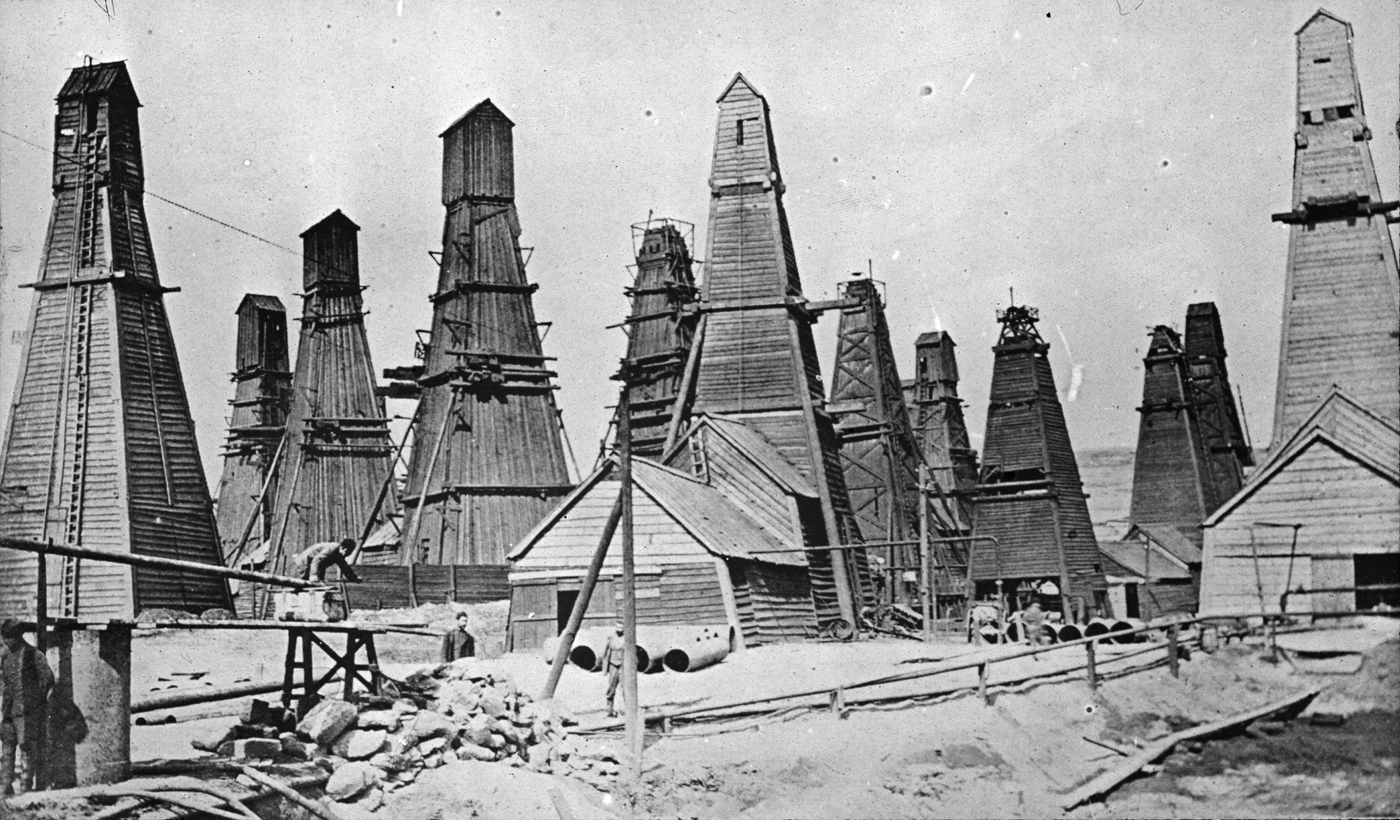
\includegraphics[width=\textwidth]{balakhani_1904.png}
  \caption{Campos Balakhani (1904)}
  \small Produção de petróleo do início do século XX.
\end{minipage}
\hfill
\begin{minipage}[t]{0.45\textwidth}
  \centering
  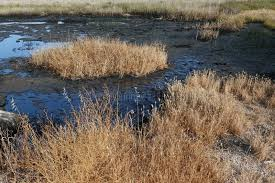
\includegraphics[width=\textwidth]{afloramento natural de betume fonte-.jpg}
  \caption{Afloramento de Betume}
  \small Emanação natural desde a Antiguidade para impermeabilização.
\end{minipage}
\end{figure}

O traço comum era a completa ausência de método: sem cálculo de volumes, sem conhecimento de pressão ou dinâmica subsuperficial. Essa primeira era (Antiguidade-XVIII) caracteriza-se pelo empirismo e ausência de fundamentação científica.

Em 1856, Henry Darcy formulou a lei que governafluxo em meios porosos. Em 1859, o poço Drake (Titusville, PA) provou viabilidade econômica. Esses marcos definem o nascimento da Engenharia de Reservatórios como disciplina científica: a lei $q = -k \frac{dP}{dx}$.

\begin{figure}[H]
\begin{minipage}[t]{0.3\textwidth}
  \centering
  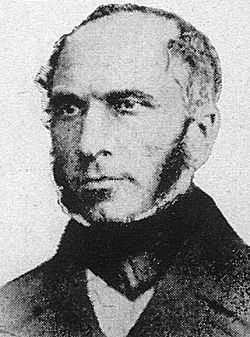
\includegraphics[width=\textwidth]{Henry_Darcy.jpg}
  \caption{Henry Darcy (1803-1858)}
  \small Engenheiro que formulou a Lei de Darcy, fundamento do fluxo em meios porosos.
\end{minipage}
\hfill
\begin{minipage}[t]{0.3\textwidth}
  \centering
  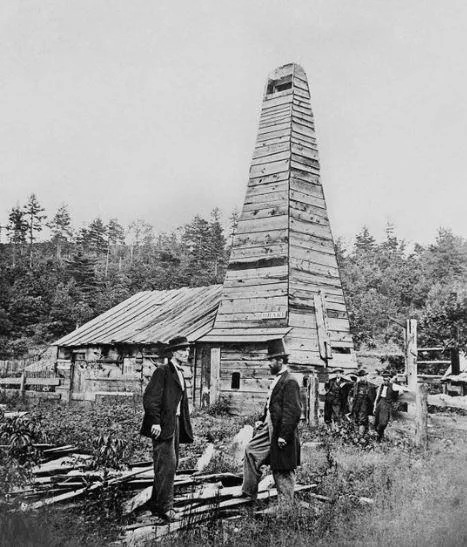
\includegraphics[width=\textwidth]{drake_well.jpg}
  \caption{Poço Drake (1859)}
  \small Primeira extração comercial bem-sucedida de petróleo em Titusville.
\end{minipage}
\hfill
\begin{minipage}[t]{0.3\textwidth}
  \centering
  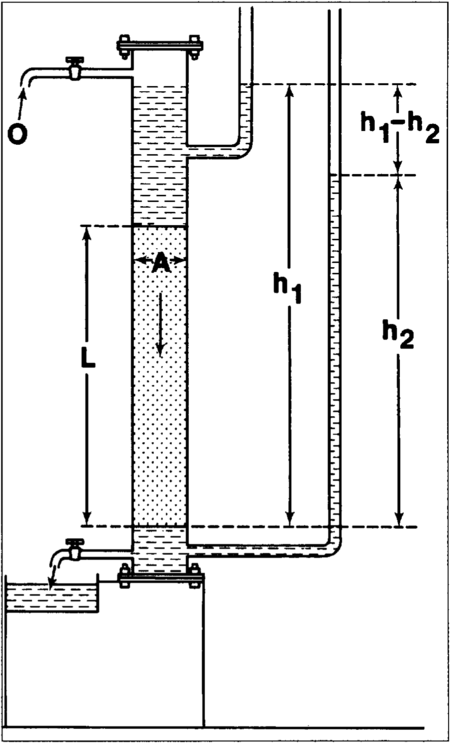
\includegraphics[width=\textwidth]{Modified schematic diagram of Darcy's experimental apparatus.png}
  \caption{Aparelho de Darcy}
  \small Demonstração experimental que validou linearidade entre pressão e fluxo.
\end{minipage}
\end{figure}

Durante essa era, desenvolvem-se os conceitos fundamentais: porosidade ($\phi$), permeabilidade ($k$), propriedades PVT, e primeiros métodos de estimativa de OOIP.

\section{Consolidação Metodológica: Balanço de Materiais, Análise Transiente e Simulação Numérica (1936-1980)}

No século XX, três pilares técnicos surgem: balanço de materiais (Schilthuis, 1936), análise de pressão transiente (Horner, 1951), e simulação numérica multifásica (1960s+). A evolução computacional foi crítica: ENIAC viabilizou cálculos complexos; CDC 7600 permitiu resolver sistemas com centenas de milhares de incógnitas.

\begin{figure}[H]
\begin{minipage}[t]{0.3\textwidth}
  \centering
  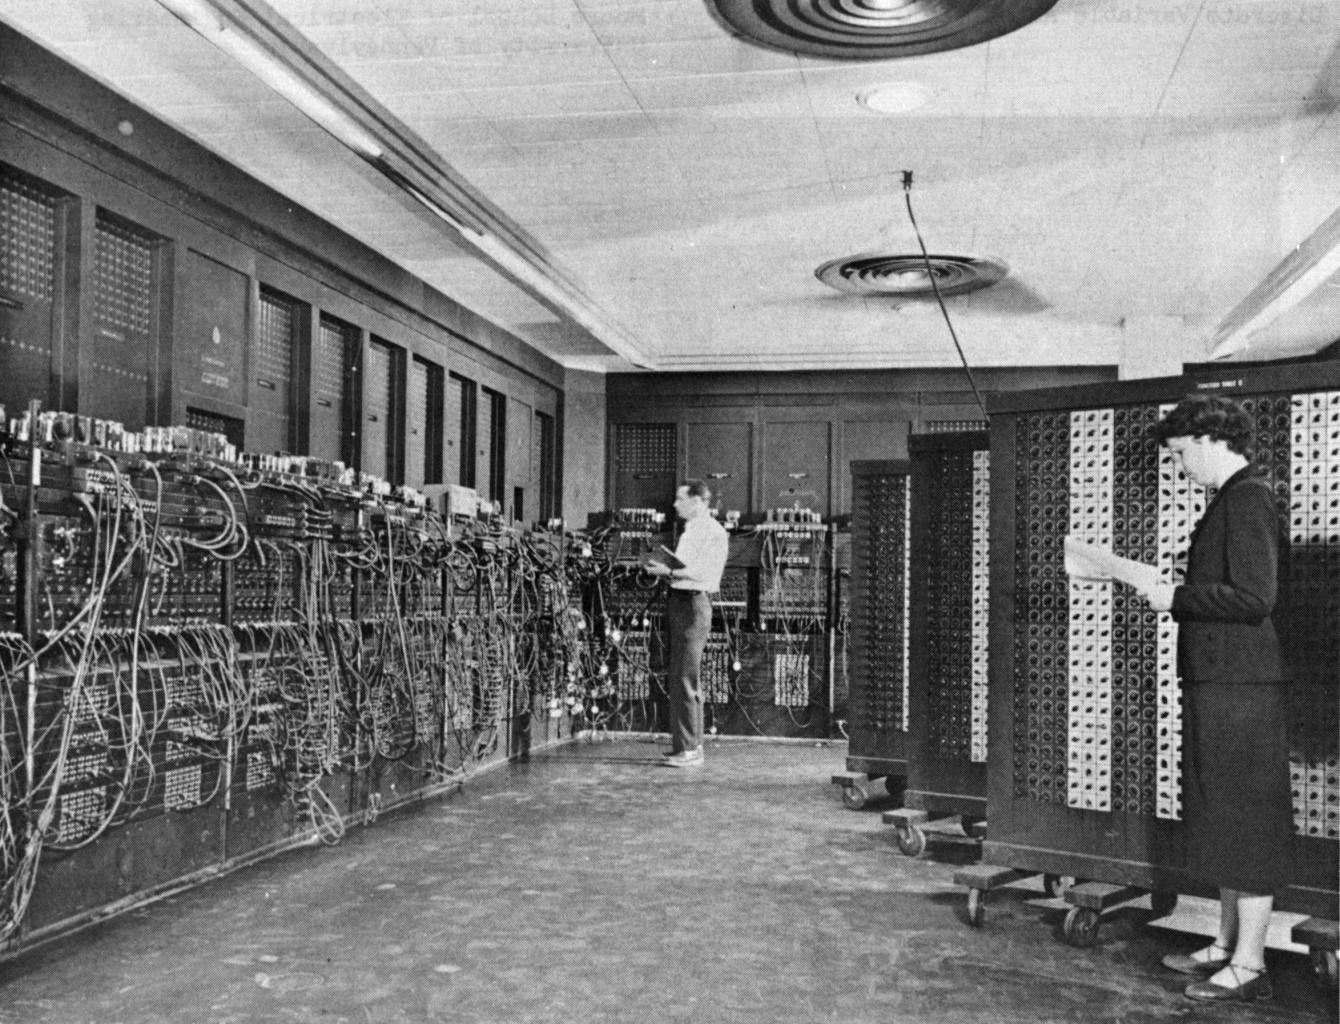
\includegraphics[width=\textwidth]{eniac_1946.jpg}
  \caption{ENIAC (1946)}
  \small Primeiro computador eletrônico de propósito geral. Viabilizou cálculos impossíveis manualmente.
\end{minipage}
\hfill
\begin{minipage}[t]{0.3\textwidth}
  \centering
  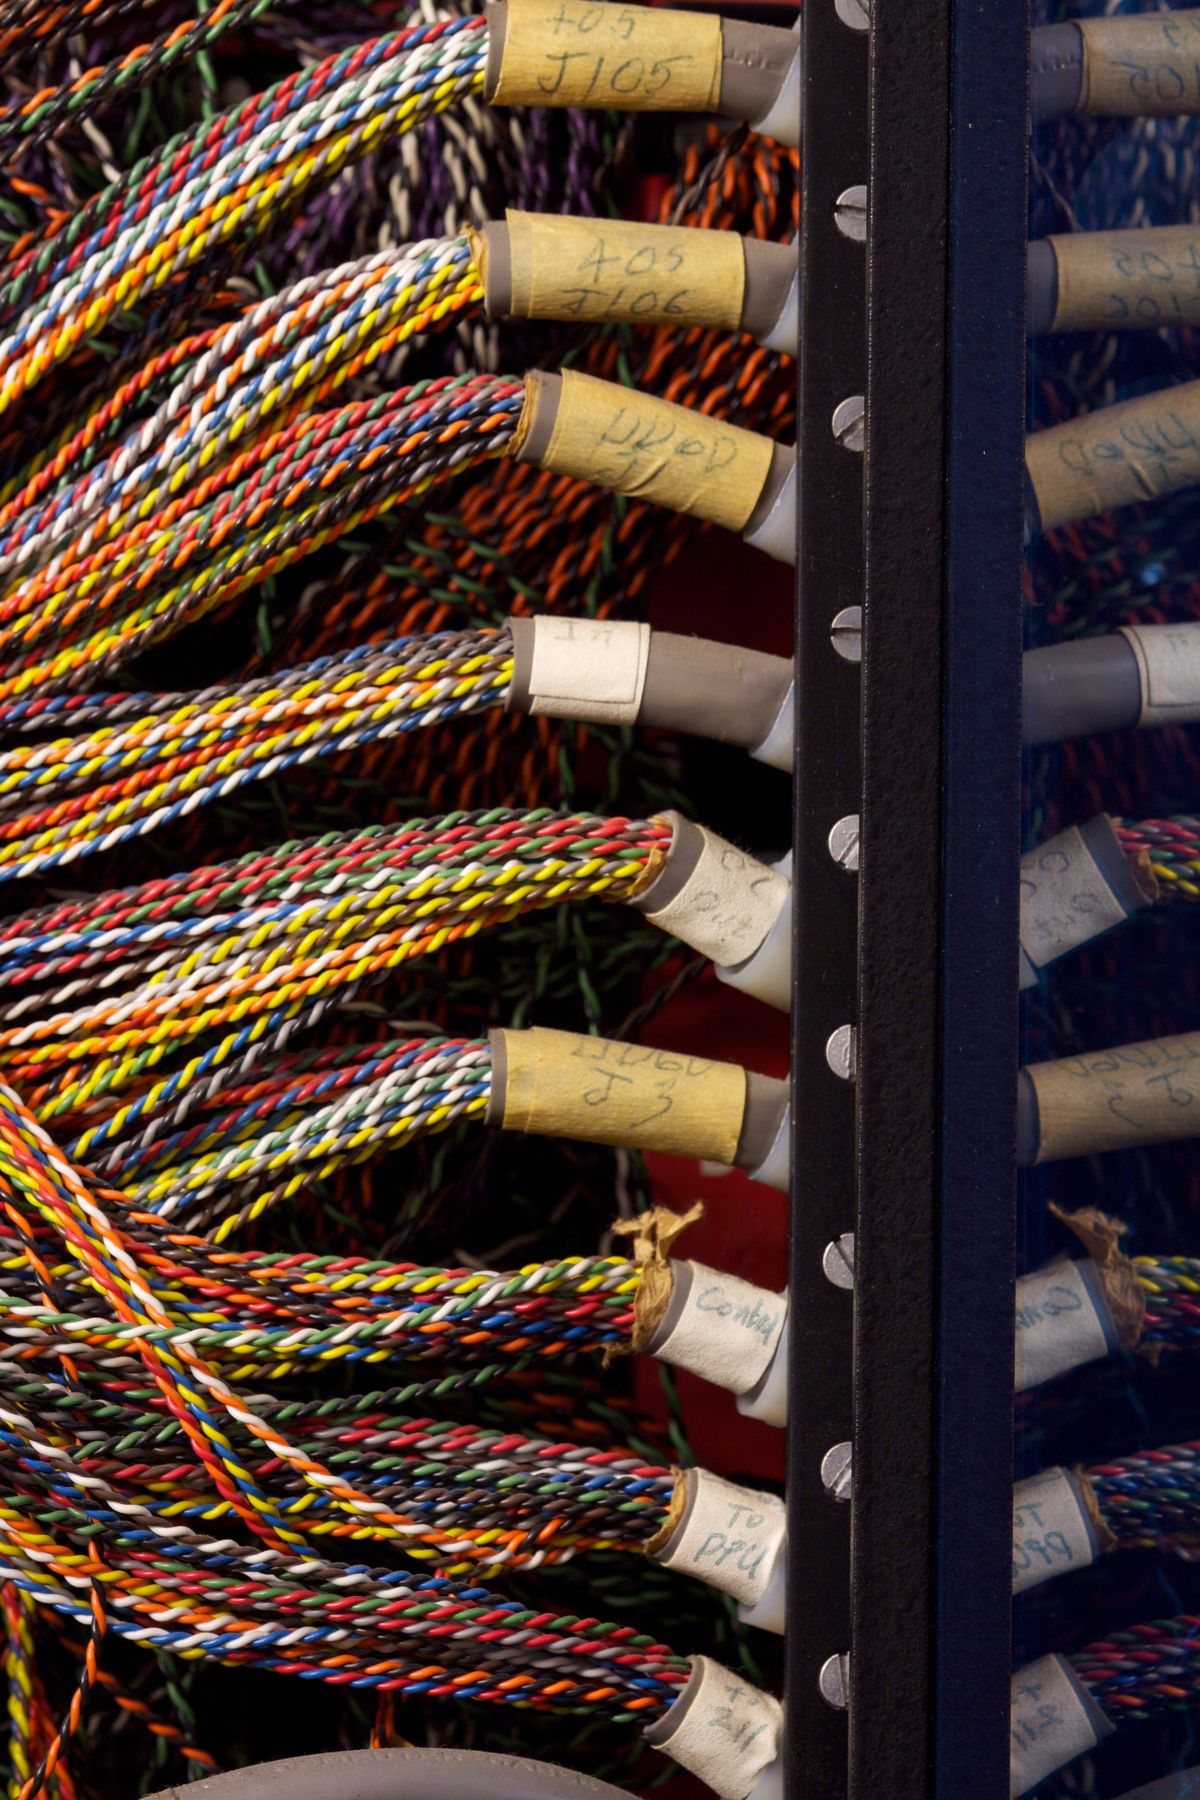
\includegraphics[width=\textwidth]{cdc_7600_1969.jpg}
  \caption{CDC 7600 (1969)}
  \small Supercomputador que permitiu simulação numérica multifásica de reservatórios complexos.
\end{minipage}
\hfill
\begin{minipage}[t]{0.3\textwidth}
  \centering
  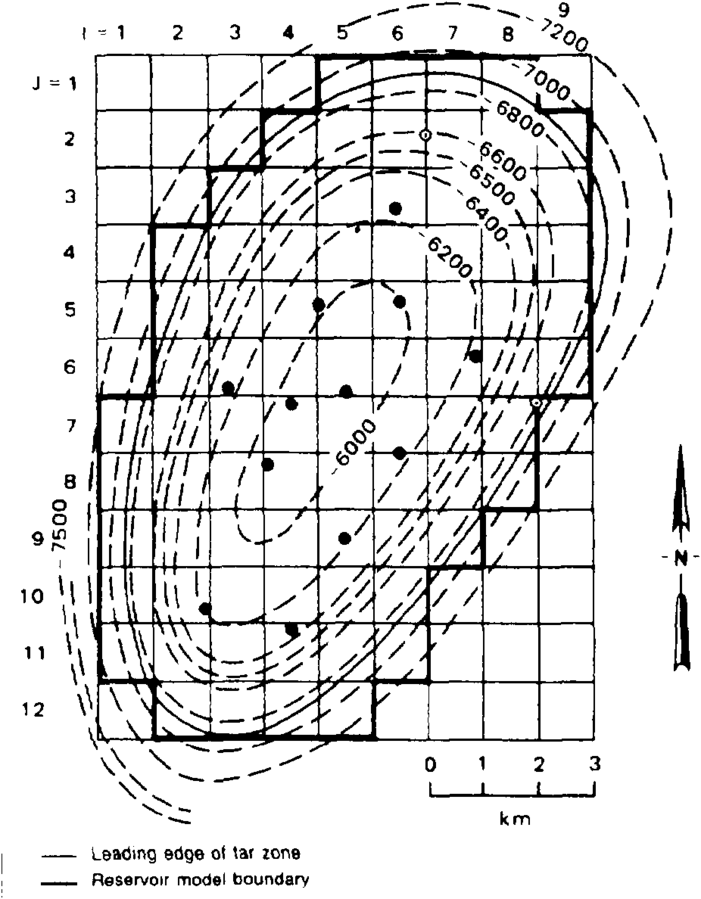
\includegraphics[width=\textwidth]{701px-Conducting-a-reservoir-simulation-study-an-overview_fig3.png}
  \caption{Malha Numérica}
  \small Discretização cartesiana para resolver equações de fluxo multifásico em subsolo.
\end{minipage}
\end{figure}

Esta era estabelece a fundamentação teórica rigorosa sobre a qual repousa toda a prática profissional moderna de engenharia de reservatórios. O balanço de materiais relaciona volumes iniciais, produzidos, e influxo de água. Análise transiente permite inferir propriedades locais. Simulação numérica integra heterogeneidade geológica.

\section{A Era Digital e Avançada: Inteligência Artificial, IoT e Otimização (1981 até Presente)}

A partir do final do século XX, a Engenharia de Reservatórios beneficia-se de três desenvolvimentos tecnológicos convergentes que transformam a prática disciplinar:

\subsection*{Internet das Coisas (IoT) e Monitoramento em Tempo Real}

Sensores distribuídos em poços e campos (medidores de pressão, temperatura, vazão, composição) permitem coleta contínua de dados de produção, retroalimentando sistemas de controle automático e decisão. Alarmes inteligentes identificam anomalias (queda anômala de pressão, surgimento de água, desvio de produtor vs. predito).

\subsection*{Aprendizado de Máquina e Análise de Dados}

Redes neurais artificiais, algoritmos de regressão não-linear e técnicas de classificação identificam padrões em históricos de produção (séries temporais de $P(t)$, $q(t)$, $S_w(t)$), permitindo:
\begin{itemize}
  \item Classificação automática de tipos de reservatório (frao-drenado, limitado, depleção-acionado);
  \item Previsão de produção futura sob diferentes cenários (velocidade de retirada, injeção);
  \item Otimização de tipo/localização de poços e quantidade de injetor versus produtor;
  \item Ajuste preditivo de modelos de simulação baseado em histórico observado (history matching).
\end{itemize}

\subsection*{Recuperação Avançada de Petróleo (EOR) e Métodos Especiais}

Técnicas sofisticadas para mobilizar óleo residual após produção primária e injeção de água:
\begin{itemize}
  \item Injeção de gás imiscível: reduz viscosidade do óleo e aumenta pressão;
  \item Injeção de polímeros e surfactantes: altera mobilidade e tensão interfacial;
  \item Alternância água/gás (WAG) e ciclos de vapor: maximiza contacto fluido-rocha;
  \item Combustão in situ: reação exotérmica aquece óleo e reduz viscosidade.
\end{itemize}

A escolha de estratégia EOR depende de avaliação técnico-econômica rigorosa de custos vs. ganho de fator de recuperação. Campos maduros de Angola (Soyo, Malongo) são candidatos prioritários para piloto de EOR.

\begin{figure}[H]
  \centering
  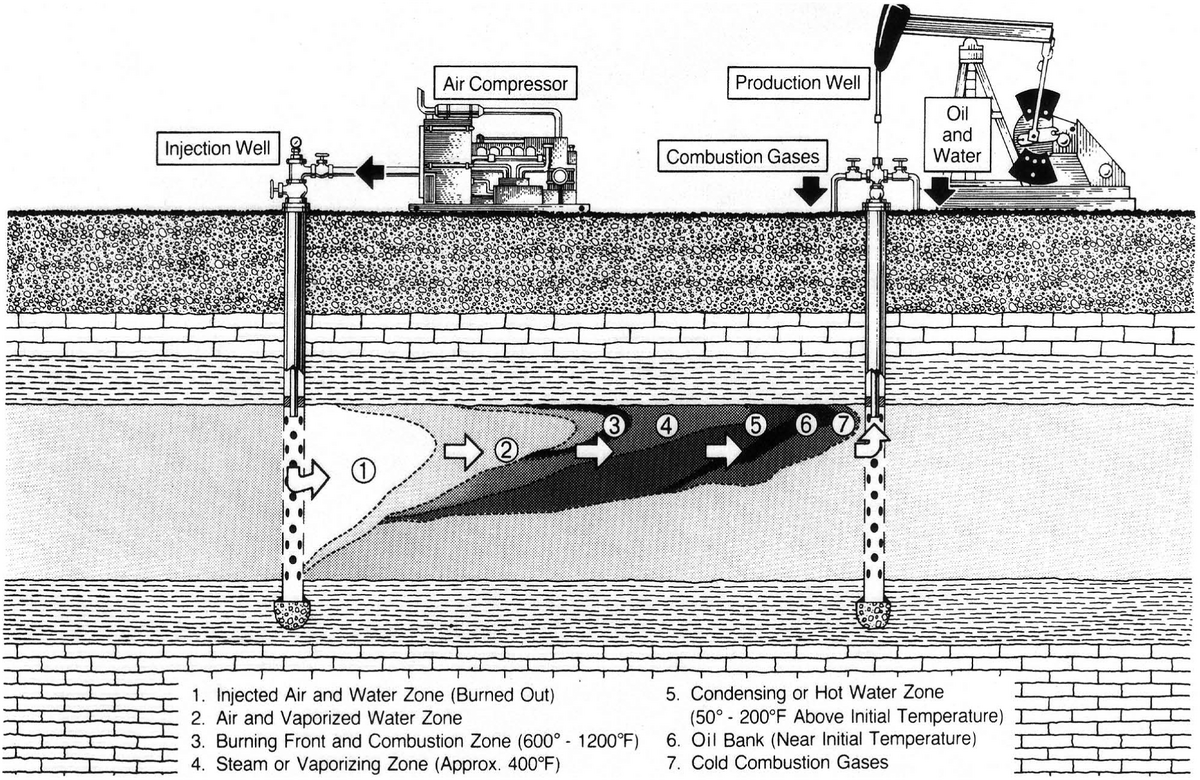
\includegraphics[width=0.4\textwidth]{Enhanced-oil-recovery.png}
  \caption{Métodos EOR}
  \label{fig:eor}
\end{figure}

Essa era não apenas integra todas as conquistas anteriores, mas as transcende, criando sistemas adaptativos de gestão de campos que aprendem com novos dados e se otimizam continuamente.

\section{Implicações para a Formação Profissional em Angola}

Angola enfrenta desafios específicos:

\begin{itemize}
  \item Campos offshore em águas profundas e ultra-profundas que exigem expertise em ambientes de alta complexidade geológica;
  \item Necessidade de maximizar recuperação de campos maduros para estender a vida produtiva do país;
  \item Imperativo de transição para modelos de exploração mais sustentáveis e alinhados com objetivos climáticos globais;
  \item Urgência de desenvolver uma base técnica e científica local que não dependa exclusivamente de expertise estrangeira.
\end{itemize}



Engenheiros capazes de gerir esses desafios — com soberania técnica, eficiência operacional, responsabilidade socioambiental, e capacidade de inovação — só podem ser formados se dominarem os fundamentos históricos e teóricos sobre os quais a Engenharia de Reservatórios foi construída.



\chapter{Conclusão}

Este trabalho traçou a trajetória histórica da Engenharia de Reservatórios de Petróleo, identificando quatro fases paradigmáticas claramente delimitadas:

1. \textbf{Era Empírica} (Antiguidade--século XVIII): Ausência completa de teoria; conhecimento transmitido oralmente; petróleo visto como recurso natural indefinido.

2. \textbf{Era da Fundamentação Teórica} (1856--1935): Nascimento científico com Lei de Darcy; primeiros modelos matemáticos; reconhecimento de que o subsolo é um sistema físico governado por princípios quantificáveis.

3. \textbf{Era da Consolidação Científica} (1936--1980): Desenvolvimento do balanço de materiais, análise de testes de pressão transiente, e primeiros simuladores numéricos; transformação de disciplina empírica em ciência quantitativa de previsão.

4. \textbf{Era Digital e Avançada} (1981--presente): Integração de IoT, aprendizado de máquina, otimização computacional, e Recuperação Avançada de Petróleo; transição de sistemas determinísticos para adaptativos baseados em dados.

A conclusão central é que a Engenharia de Reservatórios exemplifica de forma paradigmática como o conhecimento humano transita de práticas artesanais para ciência rigorosa. Os marcos teóricos (Lei de Darcy, MBE, equação de difusividade) e inovações tecnológicas (simulação numérica, sensores inteligentes, algoritmos de IA) sucedem-se segundo uma lógica clara: cada fase resolve limitações da anterior, incorporando-a como caso especial. O balanço de materiais é um caso limite da simulação numérica; a simulação numérica é discretização da equação de difusividade; os modelos de aprendizado de máquina exploram padrões em históricos de pressão-produção que as técnicas clássicas não conseguem capturar.

O desafio contemporâneo reside em manter a rigor teórico enquanto se abraça a flexibilidade dos métodos data-driven. Engenheiros capazes de fazer esta síntese — compreendendo tanto os princípios fundamentais quanto as capacidades emergentes — moldará o futuro da disciplina.

\postextual
\bibliography{referencias}

\end{document}
